\section{Implementation}

	\note{provide nice bridging}
	In this section we disuss the implementation of the suggested approach.
	First we\ldots Afterwards\ldots
	
	\begin{figure}[!t]
			\centering
				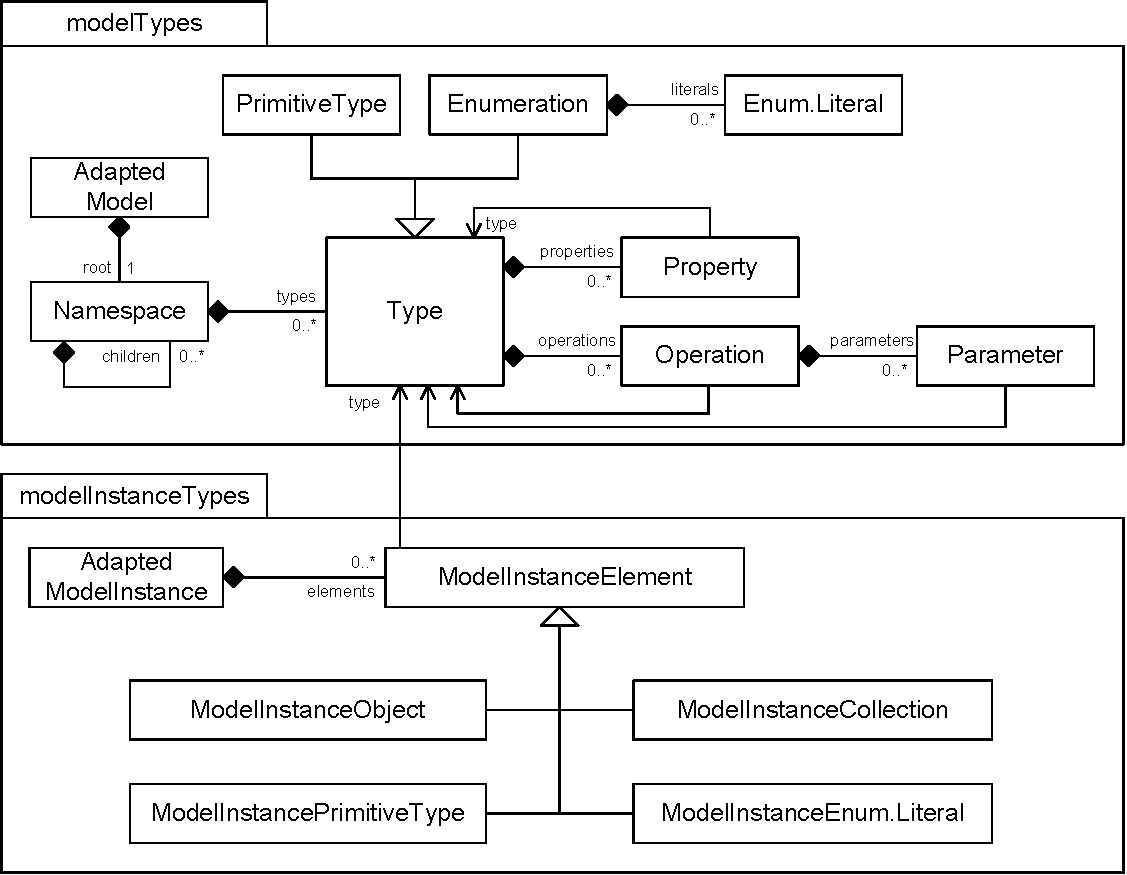
\includegraphics[width=1.00\textwidth]{figures/coreconcepts.pdf}
			\caption{The core concepts of the \textit{Model Types} and \textit{Model Instance Types}. 
			Each model \textit{Type} is located in a \textit{Namespace} and has a set of \textit{Operations} 
			and \textit{Properties}. Each \textit{Model Instance Element} has exactly one Type and provides 
			operations to reflect on this Type. \textit{Model Instance Objects} provide further reflective 
			operations to get properties or to invoke operations.}
			\label{fig:coreconcepts}
		\end{figure}

\subsection{Model Adaptation}

	\begin{figure}[tb]
			\centering
				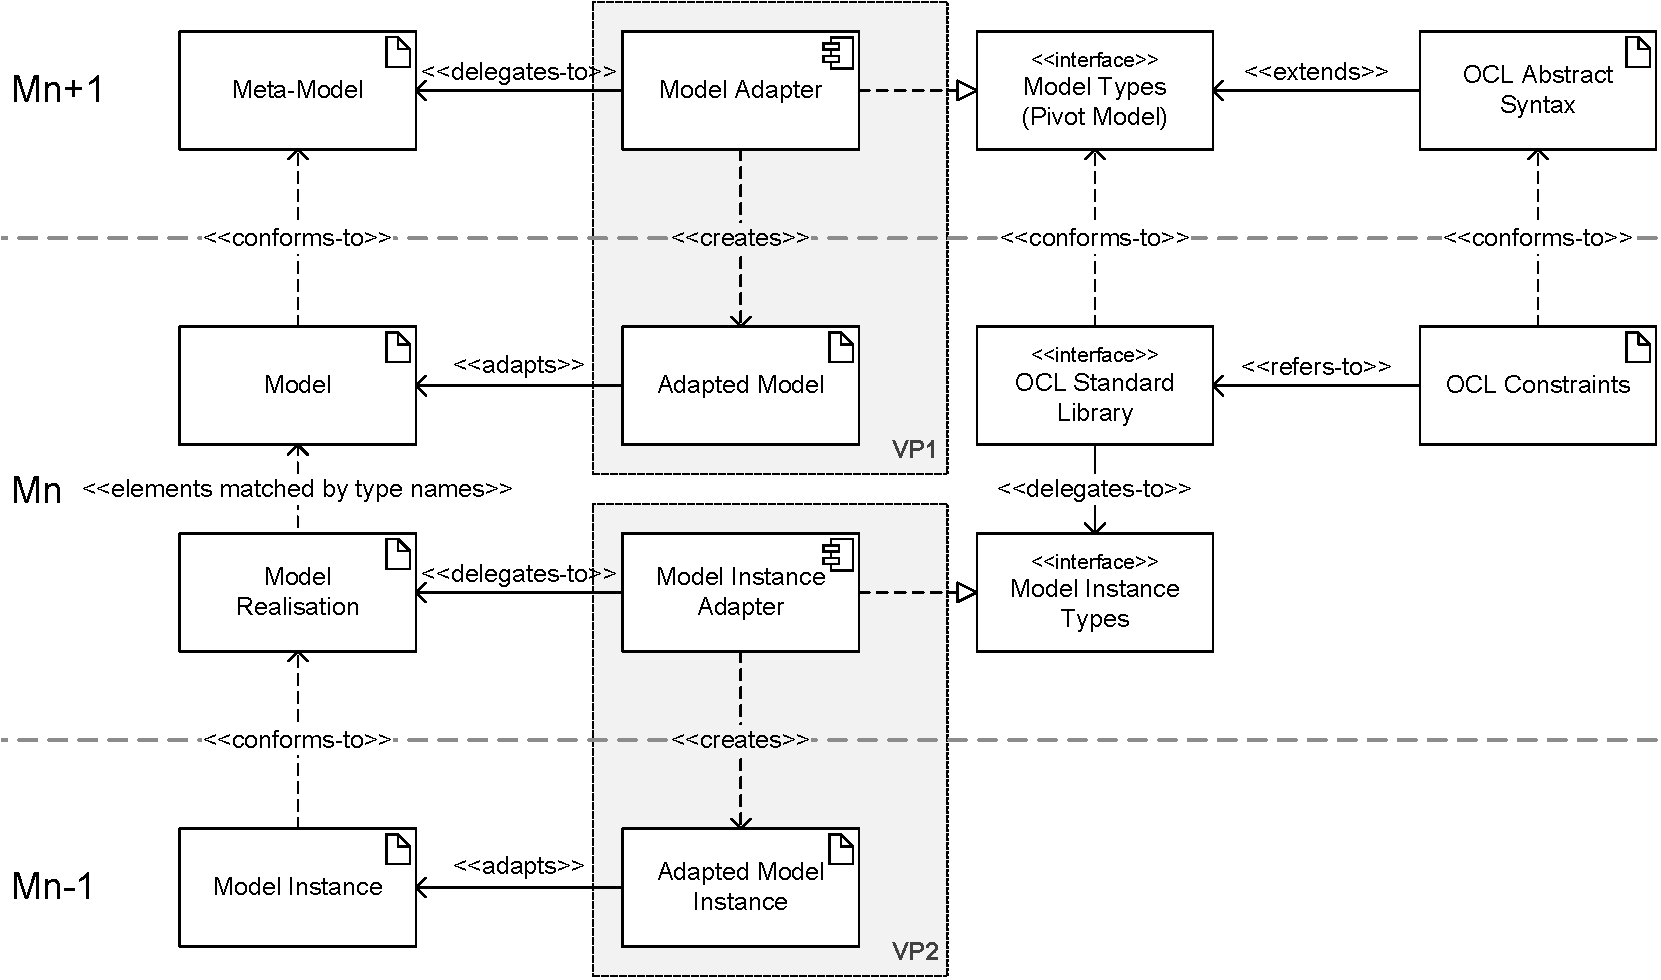
\includegraphics[width=1.00\textwidth]{figures/modeladaptation.pdf}
			\caption{\note{Claas: Relationship between OCL AS and Model Types, between Constraints 
			and Standard Library is unclear. Better relationships?}
			\note{Christian: Explain context there. inheritance relations are not explained,
			highlight adapter pattern} 
			The \textit{Generic Adaptation Architecture} of DresdenOCL: At the Mn+1 layer, meta-models are adapted
			to the model types (VP1). The model adapter component contains these adapters and is responsible 
			to instantiate them to adapt models of the meta-model. 
			At the Mn layer, model implementation types are adapted (VP2). The model instance adapter component
			contains these adapters and is responsible to instantiate them to adapt model instance objects. 
			The OCL standard library implements the logic to evaluate operations defined on OCL types. Other 
			requests such as operation invocations or property requests on adapted objects are delegated 
			via the interfaces of the model implementation type model.}
			\label{fig:modeladaptation}
		\end{figure}

	\add{To enable the definition of OCL constraints for various modeling languages
	DresdenOCL provides a common interface abstracting structures
	that are required to navigate and query object structures.} 
	%\remove{Handling
	%different types of models behind common interfaces is the basis to define
	%a generic OCL meta-model and abstract syntax that can be} 
	The
	so-called \emph{Pivot Model} \cite{braeuerOCL07} \add{standardises the basic
	concepts that bind OCL constraints to a concrete modeling languages such as types, properties,
	operations and parameters.} DresdenOCL \change{only invoke the interfaces}{only
	uses these concepts} \change{of the pivot model when they want to reason on
	types defined in the adapted
	models}{to parse and statically analyse OCL constraints, e.g., the OCL2 parser
	invokes the operation \texttt{getType()} to access the \texttt{Type} of 
	an \texttt{Operation} or \texttt{Property}}. \note{can't understand this
	example without figure} 
	\remove{Thus, the OCL2 Parser does not 
	need to know the adapted meta-model and can be connected with different 
	meta-models very easily.}
	
	For every meta-model that shall be connected with Dresden OCL2 for Eclipse, 
	a \textit{Meta-Model Adapter} has to be implemented (see Figure \ref{fig:modeladaptation}, Mn+1 layer). 
	\add{It contains individual adapters that map concepts of the modeling
	language to corresponding artefacts in the pivot model.} E.g., the UML
	meta-model concept \texttt{UMLClass} is adapted to the pivot model concept
	\texttt{Type} \note{again, figure needed}. Furthermore, the meta-model adapter
	needs to provide a factory to create adapters on demand (see Fig.
	\ref{fig:modeladaptation}, Mn+1 and Mn layer \note{don't find factory there}).
	The \remove{model element} adapters are only created when they are required and
	existing adapters are cached. Thus, we avoid unnecessary and expensive adaptation, 
	especially when working on large models of which only parts are constrained using OCL.


\subsection{Model Implementation Adaptation}
	\note{avoid footnotes, the interrupt reading flow.}
	\note{short intro that shows that now we come to our REAL contribution}
	
	Similar to the adaptation of different meta-models and models \remove{(that can
	be considered as the specification or structure of a modeled system)}, it is
	useful to \change{adapt}{hide} different model implementations
	\remove{or semantics} behind standardised interfaces. \add{This enables the
	reuse of }the same OCL2 interpreter for the \change{interpretation}{dynamic
	evaluation} of OCL constraints on model instances in various model
	implementations. \remove{Furthermore, a specific model type can have different 
	semantics in different implementations.} E.g., a UML class diagram can be
	implemented in Java, C\# or mapped to a database.\footnote{\note{I don't
	get this remark} Although the implementation of the same model in different
	programming languages is rather unusual, it is often required to connect models 
	of the same meta-model with different types of implementations.} \remove{Thus,
	it is sensible to loosely couple the models and their semantics. }
	
	\change{To fulfill these requirements}{To provide means for model
	implementation adaptation}, we introduced a the \textit{Model Implementation
	Type Model} \remove{that can be adapted to different kinds of model
	implementations.} \remove{It can be considered as similar to
	the pivot model, but has some differences as well.
	Similar to the pivot model, }The implementation type model introduces different
	interfaces for \change{different elements of an implementation such as instances
	of}{standard types in OCL such as
	primitive types, enumeration literals, collections and instances of pivot
	model concepts like Type}. All these
	interfaces inherit a common interface \textit{IModelInstanceElement}. The most 
	important difference between the pivot model and the implementation type model
	is that \texttt{IModelInstanceElements} have to provide a reflection mechanism whereas 
	pivot model elements only allow to reason on relationship between concepts of
	the same meta-level. During interpretation, the OCL2 interpreter uses this mechanism to
	retrieve the Type of a \textit{IModelInstanceElement}, access property
	values, or to invoke operations. \remove{The kind of reflection mechanism
	provided can be considered as similar to the Java 
	reflections that allow to reason on types, to cast objects and to access properties and 
	operations.}
	
	Each kind of model implementation that shall be connected with DresdenOCL is
	adapted via a \textit{Model Implementation Adapter} (see Figure
	\ref{fig:modeladaptation}, Mn layer). Similar to the meta-model adapter, 
	the model implementation adapter contains adapters that map elements of a
	concrete model instance to elements to implementation type model and has to
	provide a factory that creates \textit{Model Object Adapters} for the runtime 
	objects of the adapted implementation  (see Figure \ref{fig:modeladaptation}, Mn-1 layer). 
	A model implementation factory also 
	creates adapters for objects on demand. Adapted objects are cached to
	improve the performance and to avoid phenomenas like \textit{Object
	Schizophrenia} \note{reference}.


\subsection{Limitations of Implementation Adaptation}
	\note{Could we move this section to a later section. It is better to first
	show how cool the approach already works and then reflect on its limitations. 
	Furthermore, knowing concrete examples may help understanding the limitations}
	\note{The whole section is hard to comprehend. I would suggest to use named
	paragraphs for each concrete limitation} During the implementation of our
	generic architecture that allows connection of different types of models 
	with different types of model implementations and \note{vice versa
	direction was not introduced before}{vice versa} we met various problems and
	difficulties that are presented in this section. 

	\paragraph{Problem Name}
	As mentioned above, models and model implementations are only loosely 
	coupled to support different implementations for the same type of model.
	\note{don't understand argument: loose coupling ENABLES variable
	implementations} Thus, we have to match types of an concrete implementation to
	the types of a model. Currently, this type matching is realized by simply 
	matching the names of the types (including the names of 
	their enclosing name spaces where possible). Often, this solution is error 
	prone and further information is hidden behind our adapters that could be 
	used to improve the matching. E.g., when adapting an instance of an EMF 
	Ecore model, one could use the reflection mechanisms provided by Ecore to
	retrieve the types of EObjects. We plan to improve our matching
	that is currently scattered over multiple classes of each implementation type 
	adapter and by introducing type matching strategies that 
	can be implemented using the \textit{Chain of Responsibility} 
	pattern\cite{gamma:dp}. The chain could start by trying to match the 
	types using a implementation specific matcher and end by trying to 
	simply match the type's names as currently done.
	
	\paragraph{Problem Name}
	Another problem when using adapters for model implementation types 
	is the unwrapping mechanism of adapted elements when invoking operations 
	on the implementation's elements. E.g., to invoke an operation of a Java 
	implementation we require \texttt{Objects} as parameters instead of 
	\texttt{IModelInstanceElements}. This unwrapping mechanism is easy 
	where elements that have been adapted before are simply unwrapped 
	again. Unfortunately, during interpretation of OCL constraints, 
	new instances of primitive types or new collections can be created 
	(e.g., when invoking the OCL operation \texttt{size()} that 
	returns an \texttt{Integer} instance). Thus, the factory of a 
	model implementation adapter has to provide operations to reconvert 
	primitive types and collections to elements of the adapted model 
	instances. In some cases this can become rather complicate because 
	the adaptation between types of the implementation and the model 
	implementation type interfaces has not to be bijective. For 
	example Java \texttt{ints} and \texttt{java.lang.Integers} are 
	both mapped to \texttt{IModelInstaceIntegers}. During unwrapping, 
	the factory of the Java implementation adapter has to reflect 
	whether the method to invoke requires an \texttt{int}, an 
	\texttt{Integer} or another Java integer-like type's instance.
	 The unwrapping mechanism of an adapted implementation 
	 can be considered as the most complicate and error-prone part 
	 of the complete implementation type adaptation. \remove{Nevertheless, 
	 this part is necessary to support interpretation of OCL 
	 constraints containing operation invocations on model defined 
	 types.}\note{What are we planning to alleviate this challenge?}


	\subsection{Improving the Adaptation Process}
	\note{can we merge this with the limitations section}
	
	\paragraph{Problem Name}
	Adapting different types of meta-models\add{, models, } and model
	implementations enables the reuse of DrescenOCL for \add{various combinations
	of modeling and implementation languages}.
	Nevertheless, the adaptation process contains parts that are similar 
	for each adaptation and can be error
	prone as well. \note{how are similar and error-prone connected?}
	\note{rephrase}
	When the adaptation of a model implementation 
	type is wrong, the interpretation results may be wrong as well. 
	To improve the model adaptation process, we developed a code generator 
	for the adaptation of meta-models to the pivot model. The code 
	generator requires an annotated \change{EMF Ecore model}{metamodel} describing
	the adaptation of meta-model concepts to the pivot model concepts. 
	The code generator generates the skeleton code for all required 
	adapters and thus avoids manual implementation of these adapters. 
	For model implementation types, such a code generator is currently 
	missing.
	
	\paragraph{Problem Name}
	\remove{Furthermore,} We developed two generic JUnit test suites, 
	that can be used to test the \remove{correct} adaptation of a model 
	or model implementation, respectively. \note{Next sentence is hard to
	comprehend\ldots}The test suites require a specific test model defined in the
	adapted meta-model or a specific test implementation implemented in the 
	adapted model implementation. 
	The test suites then check if all required methods to 
	retrieve on types, operations, properties etc. are implemented 
	appropriately in respect to the specified test model or test 
	implementation. These generic test suite helped us to ensure 
	that all existing adaptations behave in the same expected manner
	and to easily detect wrong adaptations of some elements.
	\note{any future plans?}
